\subsection{Physical Kitting into Concave Conformal Cavities}
\label{subsubsec:real-negative}
%The positive cavity task provides a detailed depth image, but requires the cavity to first be presented at a flipped, 180\degree~rotation for imaging, which may not be feasible in an industrial environment. [this is a minor detail: omit. -KG 3/18]
Here, we perform the same experiment as in Section~\ref{subsubsec:real-positive}, but instead generate $I^g$ directly from an image of the cavity without flipping. Precisely, we segment out the cavity from an overhead depth image, deproject the depth image into its point cloud representation, and rotate the point cloud 180\degree~around its center of mass. Then, we project the rotated point cloud to the depth image $I^g$. %This process is illustrated in Fig.~\ref{fig:rotated-cavity}.

\begin{table}[h]
\centering
 \begin{tabular}{l c c c}\toprule
 Object & Angle & 2D Baseline & Kit-Net \\
 \midrule
 Handrail bracket & 30\degree & 0/10 & \bf 9/10 \\ 
 Ornamental handrail bracket & 30\degree & 0/10 & \bf 7/10 \\
 Sink handle & 30\degree & 1/10 & \bf 3/10 \\
 \addlinespace
 Handrail bracket & 60\degree & 0/10 & \bf 7/10 \\ 
 Ornamental handrail bracket & 60\degree & 0/10 & 0/10 \\
 Sink handle & 60\degree & 1/10 & \bf 4/10 \\
 \bottomrule
\end{tabular}
\caption{\textbf{Physical Experiments Results for Concave Cavities: }We report the number of successful kitting trials for Kit-Net and the 2D baseline over 10 trials for 3 previously unseen objects with initial rotations of 30\degree and 60\degree. Results suggest that Kit-Net significantly outperforms the baseline in all settings except for the handrail bracket with an initial rotation of 60\degree, for which neither Kit-Net nor the baseline can successfully kit the object.}
\label{table:negative-results}
\end{table}

Table~\ref{table:negative-results} shows results from experiments with 3 novel objects from Fig.~\ref{fig:clamshell-objects} across 10 controller rollouts. We observe that Kit-Net outperforms the baseline for initial rotations of both 30 and 60 degrees on the handrail bracket and sink handle, and for an initial rotation of 30 \degree for the ornamental handrail bracket. For the ornamental handrail bracket, the depth image from the concave cavity is low quality as shown in Fig.~\ref{fig:failure-modes} (center image), causing Kit-Net to fail when the object is 60 degrees away the correct insertion orientation. We examined this failure and found that it occurs because the cavity for the neck of the bracket is very thin, making it difficult to obtain a good depth image. Kit-Net also has low performance on the sink handle due to small errors in centroid matching, as discussed in the prior section. Fig.~\ref{fig:failure-modes} (bottom left) shows an example failure case where the sink handle is correctly oriented but the translation is slightly off. There were also occasional cases (Fig.~\ref{fig:failure-modes} (top left)) where the suction gripper occludes the handle of the ornamental handrail bracket. In these cases, the robot can only see the base, resulting in failure.

% \begin{figure}
  \centering
  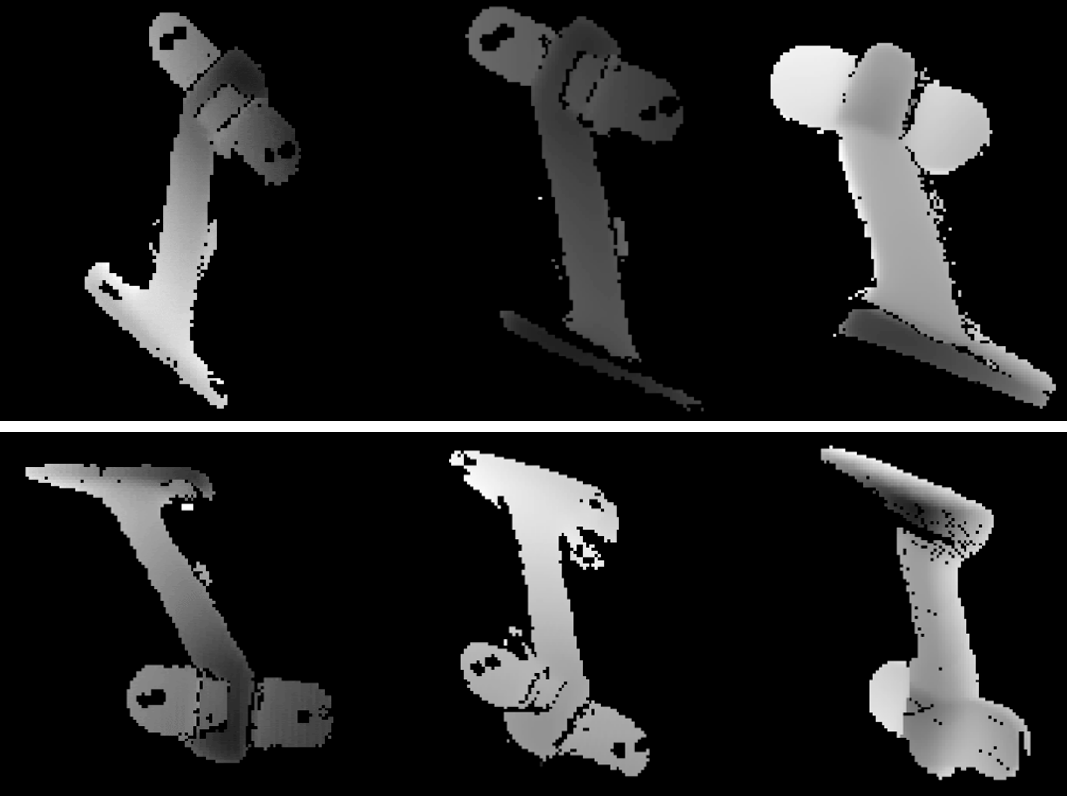
\includegraphics[width=0.48\textwidth]{figures/Orientation.PNG}
  \caption{\AB{this figure needs some labels, eg. $I^s$, $\hat{I}^g$, $I^g$}\textbf{Reorienting Objects with Kit-Net: }Kit-Net aligns objects from $I^s$ (left) to $\hat{I}^g$ (middle) given both positive (top right) and negative (bottom right) goal images $I^g$ by estimating ${_s}\hat{t}^g \in SE(3)$. Positive goal images are generated as described in Section~\ref{subsubsec:real-positive} while negative goal images are generated as described in Section~\ref{subsubsec:real-negative}.}
  \label{fig:Kit-Net-to-cavity}
\end{figure} OMIT -KG 3/18

\begin{figure}[t]
  \vspace{8pt}
  \centering
  % "Break between images" -KG
%   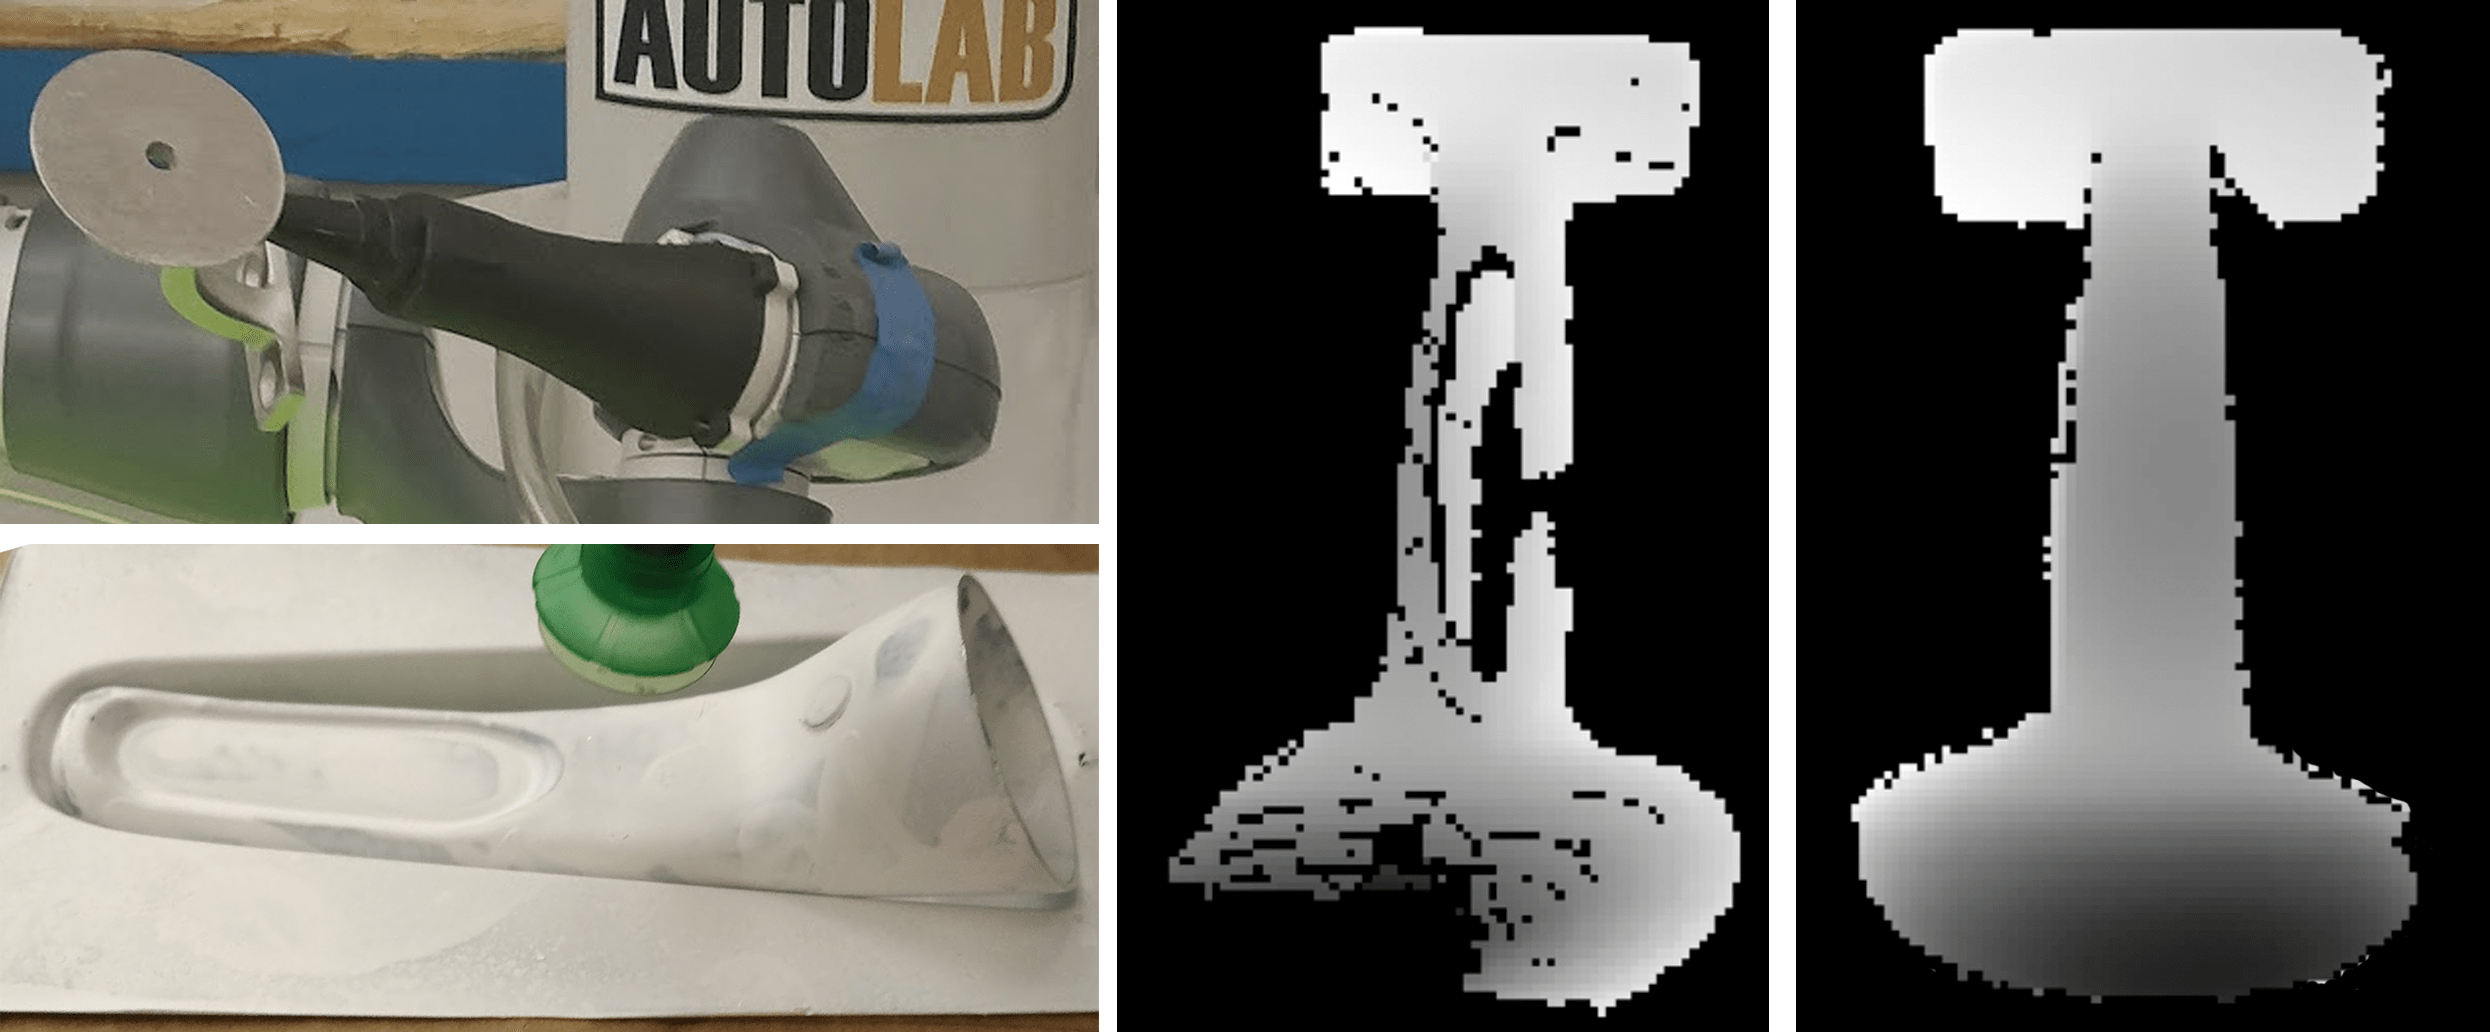
\includegraphics[width=0.48\textwidth, trim=0 488 0 0, clip]{figures/Failure Cases.png} \\[2pt]
%   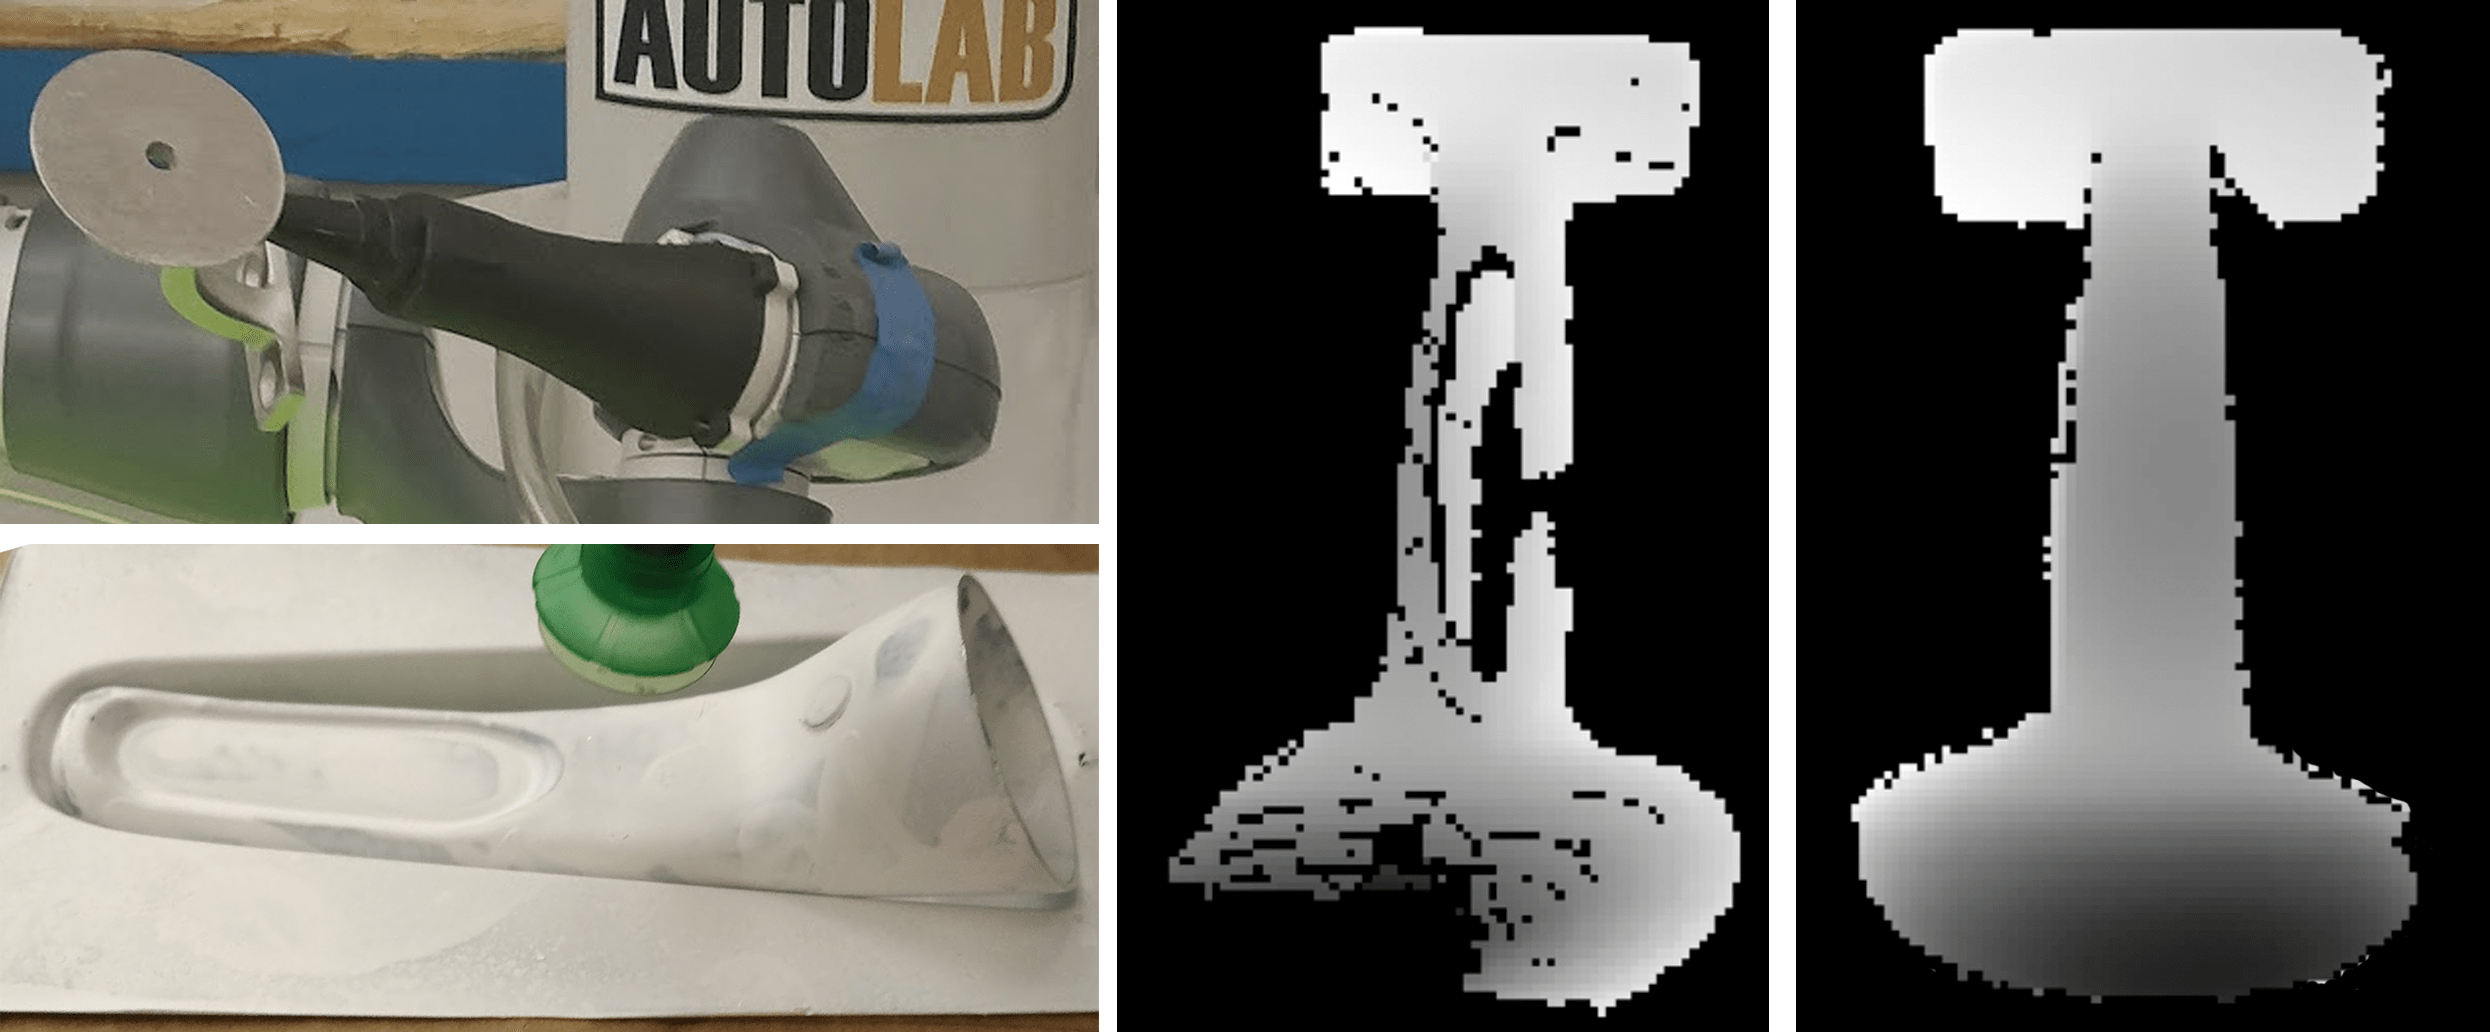
\includegraphics[width=0.48\textwidth, trim=0 0 0 636, clip]{figures/Failure Cases.png}
  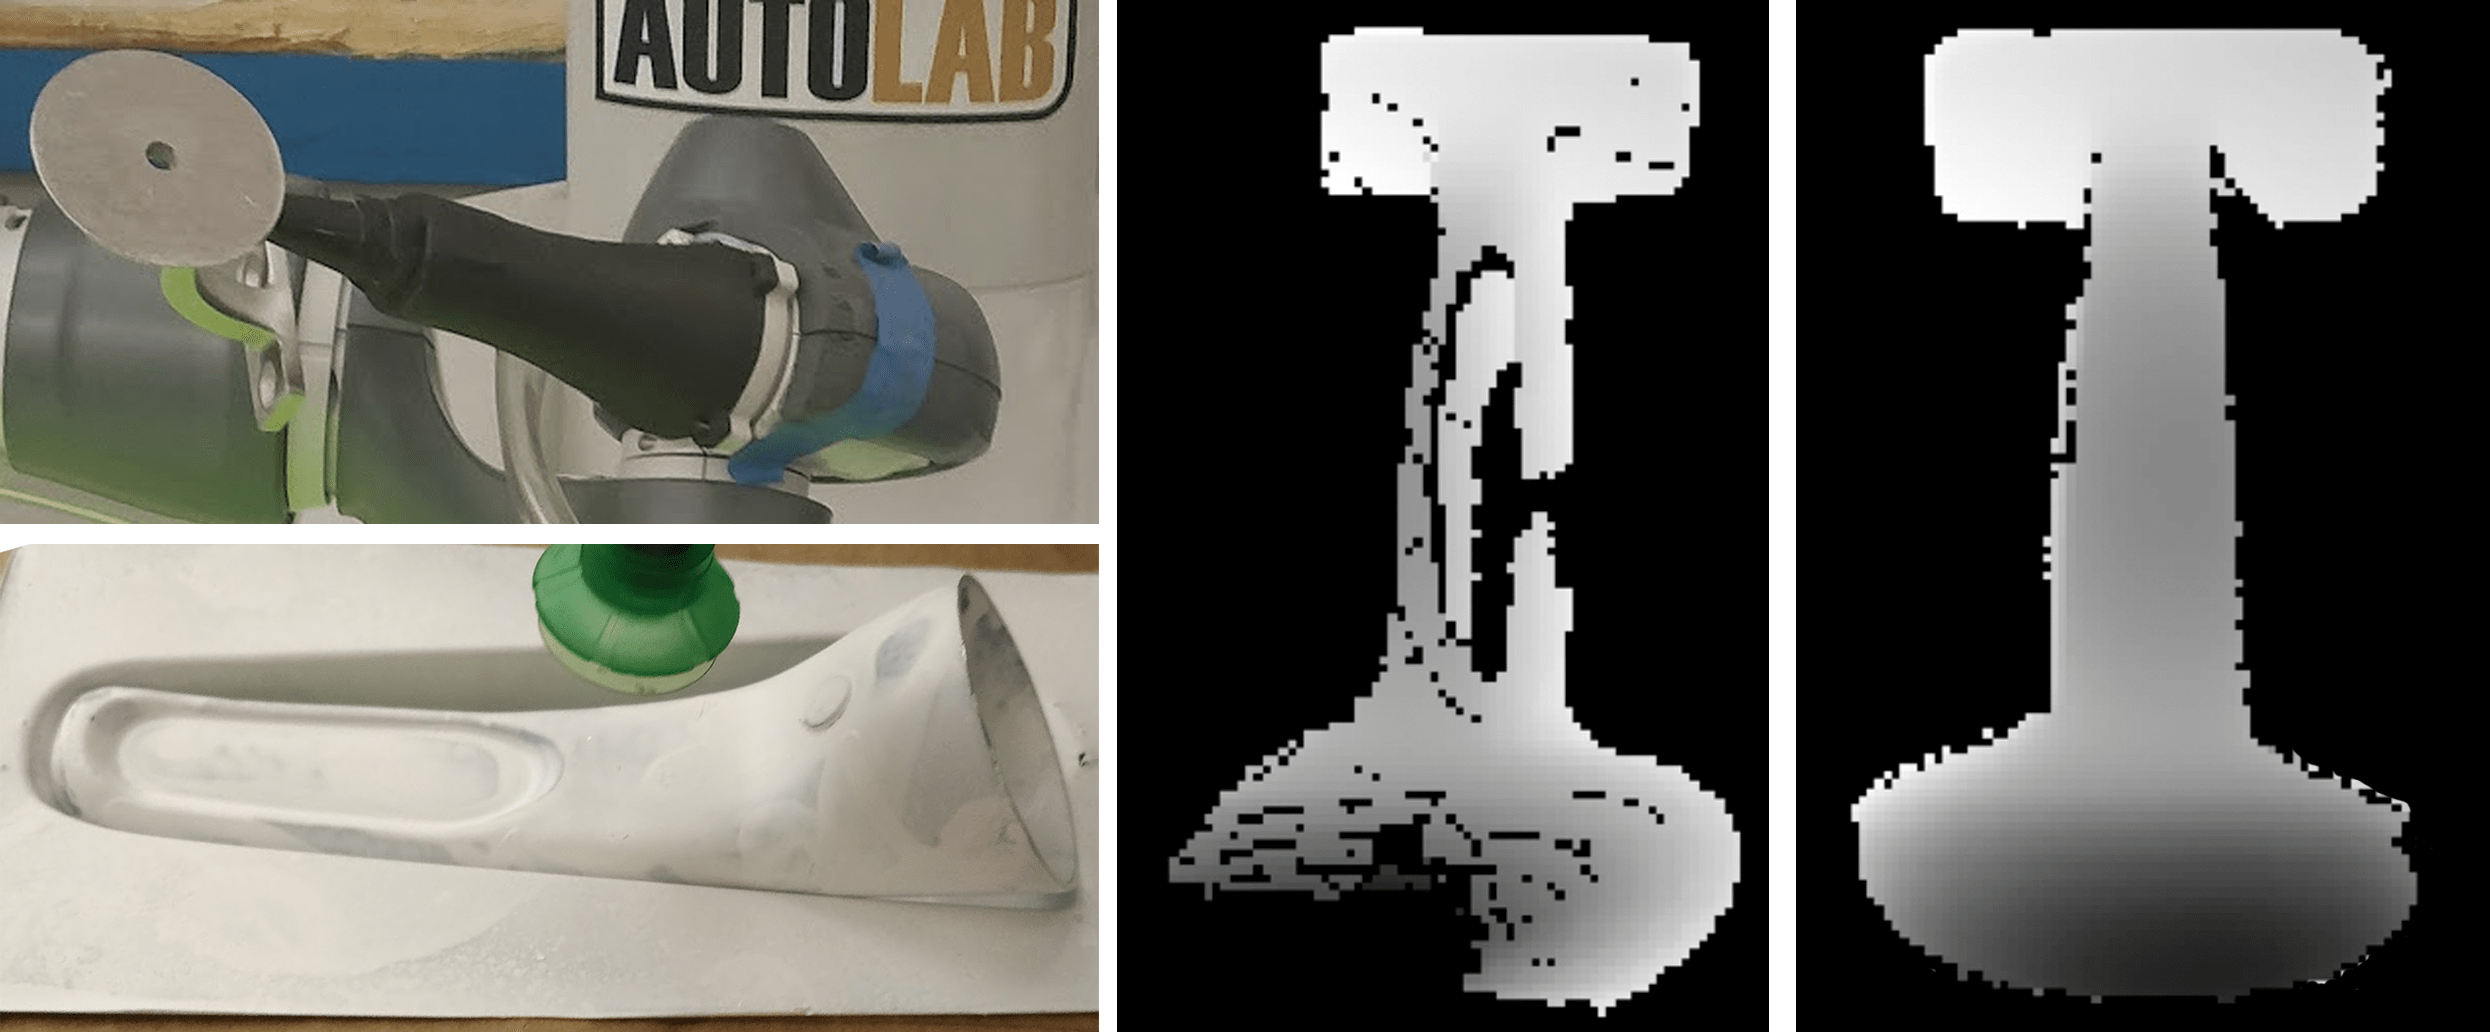
\includegraphics[width=0.48\textwidth]{figures/Failure Cases.png}
  \caption{\textbf{Kit-Net Failure Cases: } The top-left image shows a configuration of the ornamental handrail bracket
  %that results in self-occlusion; the downward-facing depth camera cannot image
  where the suction gripper occludes
  the handle below the base. The bottom-left image shows the sink handle. Although Kit-Net was able to orient the handle correctly for insertion, the centroid matching had a small error in estimating translation and the cavity does not have enough slack to be properly inserted. The center and right images show depth images for the ornamental handrail bracket for the concave conformal cavity and convex conformal cavity, respectively.
  %using the process described in \ref{subsec:real-negative}, and the right image shows the depth image of the cavity positive as described in \ref{subsec:real-positive}.
  The inside of the concave cavity is very thin and the angle of the camera makes it hard to perfectly image it, resulting in a poor depth image (center image). % using the method of \ref{subsec:real-negative}.
  This leads to 0 successes for both the baseline and for Kit-Net when the initial rotation is 60\degree{} away from the desired rotation for kitting.}
  \label{fig:failure-modes}
\end{figure}


% \begin{figure}
  \centering
  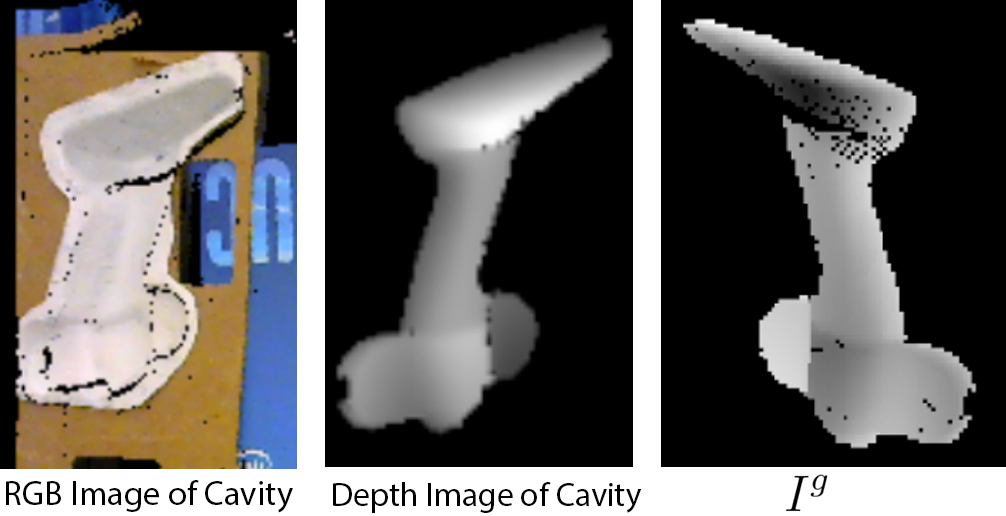
\includegraphics[width=0.48\textwidth]{figures/Rotated_Negative.png}
  \caption{\textbf{Generating Negative Goal Images: }After taking the original image (left), we segment out all parts that don't belong to the cavity (middle). Then, we project from depth to point cloud, rotate the pointcloud about its centroid, and deproject to depth image to get $I^g$ (right).}
  \label{fig:rotated-cavity}
\end{figure}
 OMIT -KG 3/18